%--------Extracción de Información
%--------Daniel Ochoa John
%--------05/06/2012

\chapter{Extracción de Información}
\label{cap:extraccion}
En este capítulo se presentará la primera parte del desarrollo realizado en este trabajo. Se mostrarán los extractores de información realizados para \textit{Twitter} y \textit{Facebook} y se explicará su funcionamiento, la forma de conexión y los documentos de salida.

\section{Extractor de información para \textit{Facebook}}
El extractor de información para Facebook es una aplicación de escritorio que fue desarrollada bajo la plataforma .NET de \textit{Microsoft}, utilizando el \textit{Framework} 4.0. Este extractor utiliza la biblioteca \textit{Facebook} C\# SDK como método de diálogo entre la aplicación y las API de esta Red Social que fueron utilizadas: \textit{Graph} API y FQL. Se procederá a analizar su funcionamiento desde dos puntos de vista: del desarrollador y del usuario final.

\subsection{Funcionamiento desde el punto de vista del desarrollador}
Desde el punto de vista del desarrollador, el funcionamiento de una aplicación creada en \textit{Facebook} implica, en primer lugar, la creación de ésta en el sitio de desarrolladores de \textit{Facebook}. En el caso del extractor de información, la aplicación creada se llama FBXML.
Cuando se crea una aplicación en \textit{Facebook}, se otorga al desarrollador dos identificadores de aplicación: el API \textit{Key}, que es el identificador único de la aplicación y el API \textit{Secret}, que es un número secreto que se otorga a la aplicación considerando los permisos de acceso a la información que ésta solicita al usuario. El API \textit{Key} es fundamental para establecer la conexión entre la aplicación de \textit{Facebook} y el extractor de información, ya que le indica con precisión a la biblioteca que aplicación de \textit{Facebook} quiere comunicarse efectivamente con el API de esta Red Social.
Posteriormente, es necesario configurar los permisos que FBXML solicitará a los usuarios para acceder a su información. Prácticamente todos los datos almacenados en \textit{Facebook} cuentan con un permiso asociado, en el caso de la aplicación utilizada en este desarrollo, la información respecto a los permisos es como se muestra en la Figura~\ref{fig:ext-im1}.

\begin{figure}
	\centering
	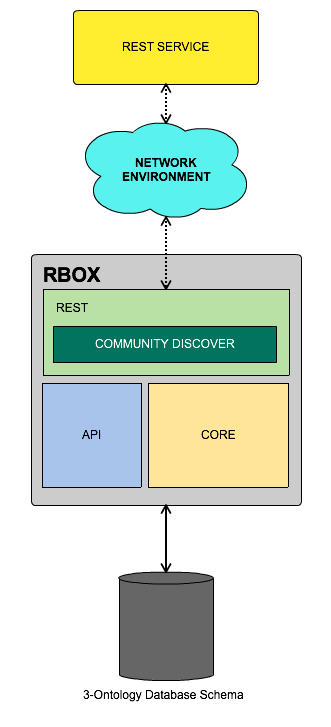
\includegraphics[scale=1]{images/Figura4-1}
	\caption{\em Permisos solicitados por FBXML.}
	\label{fig:ext-im1}
\end{figure}

Como se puede apreciar, existen dos grandes tipos de permisos: los que implican a los usuarios y sus amigos, y los permisos extendidos. Generalmente los permisos extendidos tienen que ver con la información privada en un alto grado de la palabra. Entre los permisos extendidos está \texttt{read\_mailbox}, que permite acceder a los mensajes de la bandeja de entrada del usuario. 

Para poder acceder correctamente a los datos del usuario, mediante los permisos que se definan para la aplicación, es necesario configurar el protocolo de autenticación OAuth. Para esto hay que tener en cuenta que será necesario utilizar un navegador Web para el inicio de sesión y la posterior validación de la aplicación por parte del usuario; para esto se utilizó una funcionalidad de la bibilioteca de \textit{Facebook} para C\#, el FacebookOAuthClient. Esta es una clase que permite establecer de una manera simple el protocolo OAuth para las aplicaciones. Necesita como parámetros el API \textit{Key} y un posterior análisis de los permisos. La Figura 4-2 muestra un extracto de código que representa lo anteriormente mencionado.

\begin{figure}
	\centering
	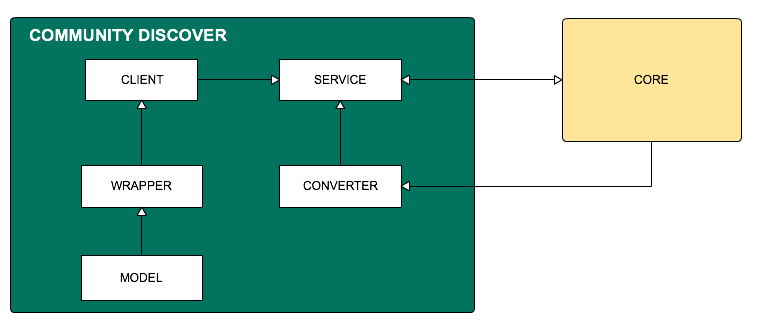
\includegraphics[scale=1]{images/Figura4-2}
	\caption{\em Configuración del protocolo OAuth en \textit{Facebook}.}
	\label{fig:ext-im2}
\end{figure}

En la línea nueve, se puede apreciar el momento de instanciar un nuevo objeto de clase FacebookOAuthClient y, como se mencionó anteriormente, el parámetro de entrada es el API \textit{Key}. El resultado de la adición de los permisos extendidos, realizado desde la línea 15 hasta la 20, permite que posteriormente, en la línea 22, se pueda obtener una dirección Web válida para utilizar como URL de inicio de sesión mediante OAuth. Es esta URL la que se deberá utilizar para redirigir al usuario para que autorice los permisos que la aplicación solicita. Ya con la aplicación configurada correctamente y con el inicio de sesión mediante OAuth creado, el siguiente paso es definir qué datos son los que se necesitan extraer.
\textit{Facebook} cuenta con una gran cantidad de datos acerca de las interacciones existentes entre dos usuarios. Esta información está repartida entre las fotografías que comparten, los mensajes enviados y los amigos en común. 

Además de lo mencionado en el capítulo anterior, respecto a que no se considerarán las publicaciones en la timeline porque aún el servicio no está implementado completamente, se suma la razón de que existe la posibilidad de que una aplicación de terceros publique contenido en la timeline de un usuario A utilizando el nombre de otro B, lo que no implica una real intención por parte de B de interactuar con A.

Para acceder a estos datos, por un asunto de conveniencia, se ha utilizado una combinación de las dos API existentes actualmente en \textit{Facebook}, \textit{Graph} y FQL. Esto es debido a que hay datos que son mucho más sencillos de conseguir utilizando una API u otra. 

En consecuencia, la información que se extraerá desde \textit{Facebook} y el método utilizado para ello se resume en la Tabla 4.1 siguiente:

\begin{table}[h]
	\begin{center}
		\caption[Datos extraídos v/s método utilizado.]{Datos extraídos v/s método utilizado}
		\label{tab:ex-tab01}
		\begin{tabular}{|c|c|}
			\hline 
			Nombre del dato & Método utilizado\tabularnewline
			\hline 
			\hline 
			Id de Facebook & Graph API\tabularnewline
			\hline 
			Nombre de usuario & Graph API\tabularnewline
			\hline 
			Fotografía de perfil & FQL\tabularnewline
			\hline 
			Amigos en común & Graph API\tabularnewline
			\hline 
			Fotografías en común & FQL\tabularnewline
			\hline 
			Tipo de relación & FQL\tabularnewline
			\hline 
			Mensajes enviados & FQL\tabularnewline
			\hline 
			Amigos del usuario. & FQL\tabularnewline
			\hline 
		\end{tabular}
	\end{center}
\end{table}

Algorítmicamente hablando, el procesamiento de la información ha sido una tarea compleja. Mientras más específico es el dato que se quiere obtener, mayor es el orden del algoritmo necesario. Un caso muy representativo es el que se presentó al momento de obtener el tipo de relación entre el usuario y sus contactos, era necesario utilizar muchas comparaciones para obtener concretamente esta información. La Figura 4-3 muestra el fragmento de código que representa esta situación.

\begin{figure}
	\centering
	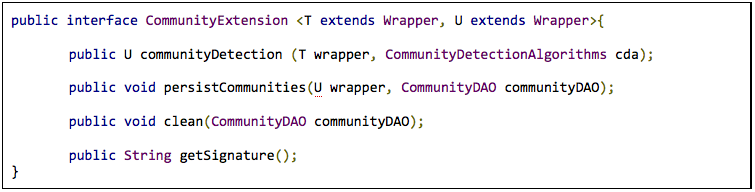
\includegraphics[scale=1]{images/Figura4-3}
	\caption{\em Obtener relaciones entre usuarios.}
	\label{fig:ext-im3}
\end{figure}

Como se puede apreciar, al existir tres ciclos foreach anidados, el algoritmo posee orden $O(n)=n^3$. La justificación de esto es lo siguiente:

En primer lugar, se obtienen todas las listas de amigos que posee el usuario en \textit{Facebook}. Luego, para cada lista, se obtienen todos los usuarios que pertenecen a esta lista. Finalmente, para cada usuario de la lista, se compara si pertenece a los amigos del usuario. 

En el apartado siguiente, se analizará el extractor desde el punto de vista del usuario.

\subsection{Funcionamiento desde el punto de vista del usuario}

El usuario tiene a su disposición un \textit{software} que explica paso a paso el procedimiento necesario para lograr el correcto uso de la herramienta. La primera \textit{screen} que aparece es la que se muestra en la Figura 4-4.

\begin{figure}[h]
	\centering
	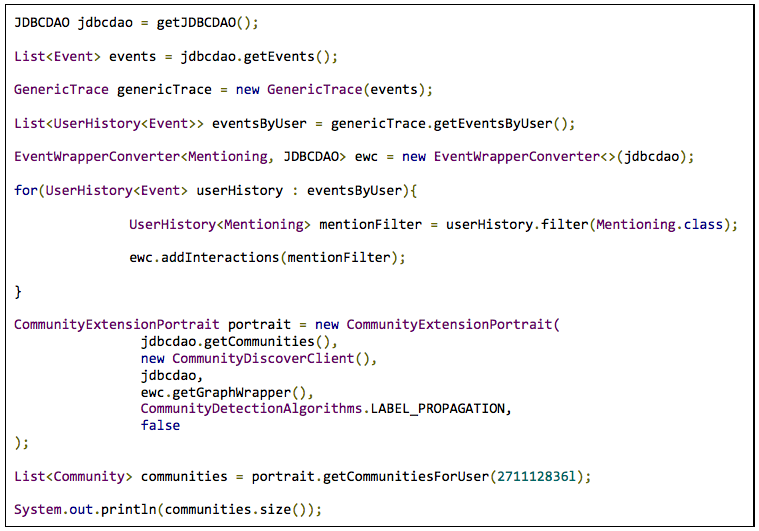
\includegraphics[scale=.7]{images/Figura4-4}
	\caption{\em Primera screen del extractor de información para Facebook.}
	\label{fig:ext-im4}
\end{figure}

Como se puede apreciar, se detallan las condiciones de uso del \textit{software} y, siempre y cuando el usuario esté de acuerdo, puede comenzar a utilizar las funcionalidades al momento de accionar el botón “Conectar Con \textit{Facebook}”. El siguiente paso es muy relevante, ya que se lleva a cabo la autenticación mediante OAuth, esto se muestra en la Figura 4-5.

\begin{figure}[h]
	\centering
	\includegraphics[scale=.7]{images/Figura4-5}
	\caption{\em Primer paso de OAuth en el extractor.}
	\label{fig:ext-im5}
\end{figure}

Como se mencionó en el apartado anterior, esta aplicación se adhiere rígidamente al protocolo de inicio de sesión seguro OAuth. En la pantalla anteriormente mostrada, el usuario es libre de conectar la aplicación con \textit{Facebook} al ingresar sus credenciales, sin embargo, esto no es suficiente.
La segunda fase de OAuth es solicitar al usuario que autorice a la aplicación de \textit{Facebook}, en la cual este extractor se sustenta (el nombre de la aplicación es FBXML), a acceder a sus datos. Esto se puede apreciar con claridad en la Figura 4-6.

\begin{figure}[h]
	\centering
	\includegraphics[scale=.7]{images/Figura4-6}
	\caption{\em Segundo paso de OAuth en el extractor.}
	\label{fig:ext-im6}
\end{figure}

\textit{Facebook} le comunica al usuario toda la información que se solicitará, que, en este caso, será la información necesaria para obtener los datos mencionados en el apartado anterior. Si el usuario responde positivamente se genera la tercera fase de OAuth, la cual se muestra en la Figura 4-7.

\begin{figure}[h]
	\centering
	\includegraphics[scale=.7]{images/Figura4-7}
	\caption{\em Tercer paso de OAuth en el extractor.}
	\label{fig:ext-im7}
\end{figure}

En esta pantalla, se solicita al usuario que permita el acceso a su información privada de alta confidencialidad. En este caso en particular ésta información está compuesta por los mensajes de la bandeja de entrada.
Si el usuario responde positivamente, el contrato mediante OAuth entre \textit{Facebook} y el extractor estará completo, se procede, entonces, a la pantalla principal, la cual se puede apreciar en la Figura 4-8.

\begin{figure}[h]
	\centering
	\includegraphics[scale=.7]{images/Figura4-8}
	\caption{\em Pantalla principal del extractor para Facebook.}
	\label{fig:ext-im8}
\end{figure}

Al momento de accionar el botón “Comenzar”, el sistema comienza la extracción y posterior procesamiento de la información. Una vez haya finalizado el proceso aparecerá un diálogo solicitando guardar en el disco duro el documento XML generado, posteriormente la aplicación se cerrará.

\subsection{Estructura del documento XML}

El documento XML que se ha generado en el proceso descrito anteriormente tiene la estructura definida considerando la información obtenida. Las etiquetas que en la Figura 4-9 se muestran, son nombres representativos para cada dato procesado. 

\begin{figure}[h]
	\centering
	\includegraphics[scale=1]{images/Figura4-9}
	\caption{\em Estructura del documento XML generado por el extractor para Facebook.}
	\label{fig:ext-im9}
\end{figure}


\section{Extractor de información para \textit{Twitter}}

El extractor de información para Twitter es una aplicación de escritorio que fue desarrollada bajo Java, utilizando el JDK 6. Este extractor utiliza la biblioteca Twitter4J como método de diálogo entre la aplicación y las API de esta Red Social. Se procederá a analizar su funcionamiento desde dos puntos de vista: del desarrollador y del usuario final.

\subsection{Funcionamiento desde el punto de vista del desarrollador}

El desarrollar una aplicación que interactúe con \textit{Twitter} implica más que sólo programar, ya que adicionalmente se vuelve imperante generar un puente entre nuestra aplicación y la Red Social. Un extremo del puente es, por supuesto, nuestra aplicación con todas sus funcionalidades, además de la API de \textit{Twitter} para facilitar la comunicación; el otro extremo es una aplicación de \textit{Twitter}. Éstas aplicaciones,símil a lo que ocurre con \textit{Facebook}, permiten a los desarrolladores acceder a la información existente en la Red Social. Es por esto que, entonces, para desarrollar el extractor de información respectivo a \textit{Twitter}, es necesario, en primer lugar, contar con una aplicación de \textit{Twitter}. La manera de realizar esto es utilizar una cuenta registrada en la Red Social, personal o corporativa, y acceder al sitio de desarrolladores para posteriormente crear una aplicación. La pantalla de creación de aplicaciones se muestra en la Figura 4-10.

\begin{figure}[h]
	\centering
	\includegraphics[scale=.5]{images/Figura4-10}
	\caption{\em Creación de una aplicación en Twitter.}
	\label{fig:ext-im10}
\end{figure}

En la Figura 4-10, se muestran los datos requeridos para crear una aplicación. En este ejemplo en particular, se adoptará \textit{Playground} como nombre de aplicación. 
Cuando se crea una aplicación en \textit{Twitter}, se hace entrega al desarrollador dos valores que funcionan como identificadores únicos de la aplicación creada: el \textit{Consumer key}, que es el identificador único de la aplicación y el \textit{Consumer secret}, que es un número secreto que se otorga a la aplicación considerando los permisos de acceso a la información que ésta solicita al usuario. El \textit{Consumer key} es fundamental para establecer la conexión entre la aplicación de \textit{Twitter} y el extractor de información, ya que representa a los cimientos de la edificación del puente entre el extractor y la Red Social.

La Figura 4-11 siguiente muestra los datos de la aplicación que se ha creado, los valores de \textit{Consumer key} y \textit{Consumer secret} han sido censurados para proteger la integridad de la aplicación. Es muy importante notar que la aplicación tiene un nivel de acceso de sólo lectura (en la imagen, \textit{Read Only}), lo que implica que todos las aplicaciones que se conecten a \textit{Twitter} a través de \textit{Playground} solamente podrán leer información y no crear ni modificar la ya existente.

Se hace necesario configurar la autenticación mediante OAuth con la finalidad de terminar de crear el puente entre el extractor de \textit{Twitter} y la aplicación creada en \textit{Twitter}. Para esto se deben utilizar dos bibliotecas: Twitter4J para manejar la conexión con \textit{Twitter} y BrowserLauncher, API creada por Chapman (2007), para manejar la interacción con el navegador Web. El siguiente fragmento de código muestra la implementación de una autenticación mediante OAuth en lenguaje Java (Figura 4-12).

\begin{figure}[h]
	\centering
	\includegraphics[scale=.5]{images/Figura4-11}
	\caption{\em Datos de la aplicación de Twitter creada.}
	\label{fig:ext-im11}
\end{figure}


Luego de asignar los valores para \textit{Consumer key} y \textit{Consumer secret} (línea censurada en la imagen), se genera un \textit{token} de petición (\textit{Request} \textit{token}). Este \textit{token} es el que permite obtener la URL de autenticación para llevar a cabo el protocolo OAuth. Esta URL es la que se abre en el navegador Web y se espera que el usuario ingrese un código que se genera al momento de que autorice a la aplicación. Finalmente, con el \textit{token} de petición y el código del usuario se genera el \textit{token} de acceso (\textit{Access} \textit{token} en la imagen), permitiendo al extractor de información comunicarse de manera efectiva con \textit{Twitter}. La interacción con el usuario de lo recientemente descrito se mostrará en el apartado siguiente.

\begin{figure}[h]
	\centering
	\includegraphics[scale=.8]{images/Figura4-12}
	\caption{\em Implementación de OAuth en Java, para Twitter.}
	\label{fig:ext-im12}
\end{figure}

Al contrario de lo que sucede con \textit{Facebook}, en \textit{Twitter} la información respecto a los usuarios, personalmente hablando, no es significativa. \textit{Twitter} es una Red Social que mayormente provee datos respecto a las tendencias de opinión de las personas, o grupos de personas. Teniendo en cuenta esto, y considerando que ésta es la segunda Red Social más popular en nuestro país, se decide extraer la información acerca de la cantidad de menciones existentes en \textit{Twitter} entre un usuario y los contactos que el sigue como métrica de interacción. La Figura 4-13 muestra un extracto de código Java en el que se observa precisamente ese proceso, obtener las menciones existentes entre el usuario y sus seguidores. 

\begin{figure}[H]
	\centering
	\includegraphics[scale=1]{images/Figura4-13}
	\caption{\em Proceso de obtener menciones.}
	\label{fig:ext-im13}
\end{figure}

El funcionamiento es el siguiente: en primer lugar, el proceso se repite para cada tweet obtenido previamente. Luego, se analiza buscando el caracter @, que es símbolo de mención a un usuario. Cuando se encuentra el caracter, se obtiene el nombre de usuario del contacto que está siendo referenciado y luego se retorna.Finalmente, el método invocador recibe ese dato y lo asigna a una lista que guarda a los usuarios y la cantidad de veces que han sido mencionados. El código respectivo al método invocador, en donde se ilustra el proceso global, se puede apreciar en la Figura 4-14.

\begin{figure}[H]
	\centering
	\includegraphics[scale=1]{images/Figura4-14}
	\caption{\em Analizar tweets.}
	\label{fig:ext-im14}
\end{figure}



\subsection{Funcionamiento desde el punto de vista del usuario}

Desde el punto de vista del usuario, el funcionamiento es intuitivo y la aplicación se encarga de guiar al usuario en todo momento. La primera pantalla que ve el usuario al iniciar la aplicación es la que muestra la Figura 4-15. Al accionar el botón “Conectar con Twitter”, se pone en marcha el procedimiento de autenticación mediante OAuth. Se dispara el navegador Web y en él aparece el diálogo de autorización de aplicaciones, como muestra la Figura 4-16. Al mismo tiempo, el validador ha desplegado un diálogo solicitando el código que se genera al aceptar la aplicación (ver Figura 4-17).

\begin{figure}[H]
	\centering
	\includegraphics[scale=.9]{images/Figura4-15}
	\caption{\em Primera pantalla del extractor para Twitter.}
	\label{fig:ext-im15}
\end{figure}

Si en el diálogo de la Figura 4-17 el usuario selecciona aceptar, se genera el código de autorización para la aplicación. Este código debe ser proporcionado al cuadro de diálogo solicitante para completar el contrato mediante OAuth. 

\begin{figure}[H]
	\centering
	\includegraphics[scale=.6]{images/Figura4-16}
	\caption{\em Diálogo de autorización de aplicaciones.}
	\label{fig:ext-im16}
\end{figure}

\begin{figure}[H]
	\centering
	\includegraphics[scale=1.3]{images/Figura4-17}
	\caption{\em Diálogo en espera de código.}
	\label{fig:ext-im17}
\end{figure}


La Figura 4-18 muestra la generación del código de autorización y su asignación al diálogo solicitante. Finalmente, se accede a la ventana principal del extractor, que muestra la Figura 4-19. Si se acciona el botón “Comenzar a escribir!” el extractor comienza el proceso de recolección y análisis de los datos existentes. 

\begin{figure}[H]
	\centering
	\includegraphics[scale=.9]{images/Figura4-18}
	\caption{\em Código de autorización.}
	\label{fig:ext-im18}
\end{figure}

Cuando el procedimiento termine, se creará un nuevo documento XML con la información obtenida, que será almacenado en el mismo directorio en el que se encuentra la aplicación y tendrá como nombre datos.xml. Luego de esto, la aplicación se cerrará.

\begin{figure}[H]
	\centering
	\includegraphics[scale=.7]{images/Figura4-19}
	\caption{\em Pantalla princpial del extractor.}
	\label{fig:ext-im19}
\end{figure}

\subsection{Estructura del documento XML}

El documento XML que se ha generado en el proceso descrito anteriormente tiene la estructura definida, considerando la información obtenida. Al igual que en caso del extractor de \textit{Facebook}, las etiquetas, que en la Figura 4-20 se muestran, son nombres representativos para cada dato procesado.

\begin{figure}[H]
	\centering
	\includegraphics[scale=1]{images/Figura4-20}
	\caption{\em Estructura del documento XML generado por el extractor para Twitter.}
	\label{fig:ext-im20}
\end{figure}


